\documentclass[10pt, unicode]{beamer}
\usepackage{fontspec}
\usepackage{polyglossia}
\setdefaultlanguage{english}
\usepackage{graphics}
\usepackage{graphicx}
\usepackage{subcaption}
\usepackage{float}
\usepackage{caption}
\usepackage{newfloat}
\usepackage{algorithm}
\usepackage{algpseudocode}
\usepackage{multirow}

\graphicspath{{images/}}
\newenvironment{algo}[1][]
  {\begin{algorithm}[#1]
     \selectlanguage{english}
     \floatname{algorithm}{Алгоритм}
  }
  {\end{algorithm}}
\DeclareMathOperator{\sech}{sech}
\setsansfont{Fira Sans}
\title{Полигонизация текстур и упаковка полигональных текстур в атлас}
\author[Терехов Д.Е.]{Студент группы М9119-09.04.01ИИБД Терехов Дмитрий Евгеньевич\\
Руководитель:\\
Старший преподаватель кафедры информатики, математического и компьютерного моделирования\\
Александр Сергеевич Кленин}
\date{26 июня 2021}
\usetheme[progressbar=frametitle, numbering=fraction]{metropolis}
\makeatletter
        \setlength{\metropolis@progressinheadfoot@linewidth}{2pt}
    \makeatother
\begin{document}
    \begin{frame}[fragile]
        \titlepage
        \thispagestyle{empty}
    \end{frame}
    \begin{frame}
        \frametitle{Отрисовка изображения}
        \begin{figure}[H]
            \centering
            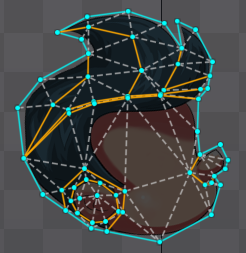
\includegraphics[scale=0.6]{spine_mesh.png}
        \end{figure}
    \end{frame}
    \begin{frame}
        \frametitle{Отрисовка изображения}
        \begin{figure}[H]
            \centering
            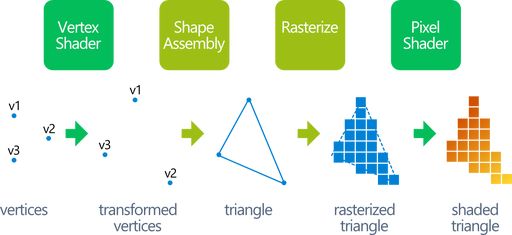
\includegraphics[scale=0.5]{graphicspipeline.png}
        \end{figure}
    \end{frame}
    \begin{frame}
        \frametitle{Текстурный атлас}
        \begin{figure}[H]
            \centering
            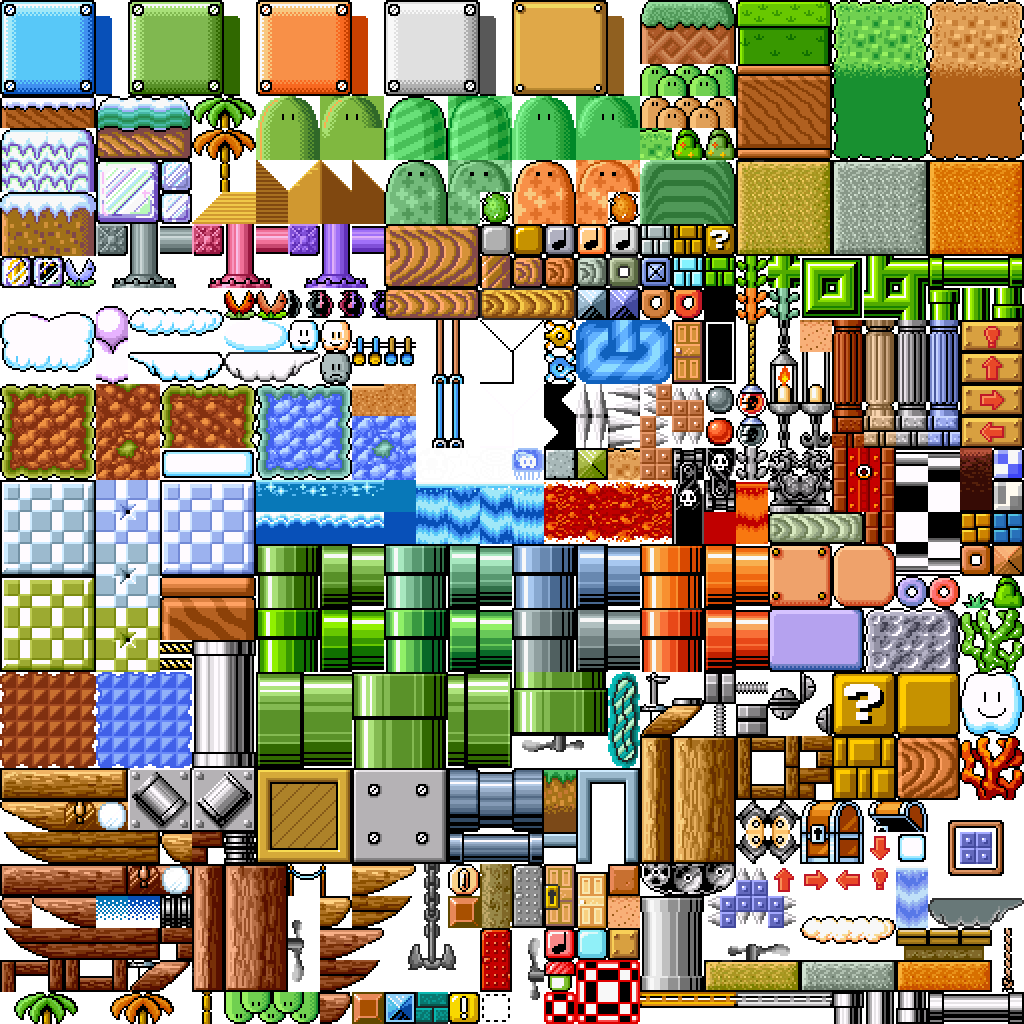
\includegraphics[scale=0.2]{texture_atlas_example.png}
        \end{figure}
    \end{frame}
    \begin{frame}
        \frametitle{Цели и задачи}
        Цель: оптимизировать отрисовку в играх (уменьшить overdraw, pixel shader invocations и количество разрыва батчей) и уменьшить размер бандла

        Задачи:
        \begin{itemize}
            \item Разработать алгоритм генерации текстурного меша
            \item Разработать алгоритм упаковки полигональных текстур в атлас
        \end{itemize}
    \end{frame}
    \begin{frame}
        \frametitle{Этапы полигональной упаковки в атлас}
        \begin{itemize}
            \item Трассировка контура
            \item Аппроксимация контура
            \item Генерация меша
            \item Упаковка в атлас
        \end{itemize}
    \end{frame}
    \begin{frame}
        \frametitle{Меш и полигоны}
        \begin{figure}[H]
            \centering
            \begin{subfigure}[t]{.49\linewidth}
                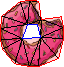
\includegraphics[scale=1.5]{donutpixel_mesh.png}
            \end{subfigure}
            \begin{subfigure}[t]{.49\linewidth}
                \centering
                
\includegraphics[scale=1.5]{donutpixel_approx_mid.png}
            \end{subfigure}
        \end{figure}
    \end{frame}
    \begin{frame}
        \frametitle{Трассировка контура}
        Алгоритм Suzuki Satoshi %\cite{SuzukiAlgorithm}
        \begin{figure}[H]
            \centering
            \begin{subfigure}[t]{.49\linewidth}
                \centering
                
\includegraphics[scale=0.25]{SuzukiExample_upscaled.png}
            \end{subfigure}
            \begin{subfigure}[t]{.49\linewidth}
                \centering
                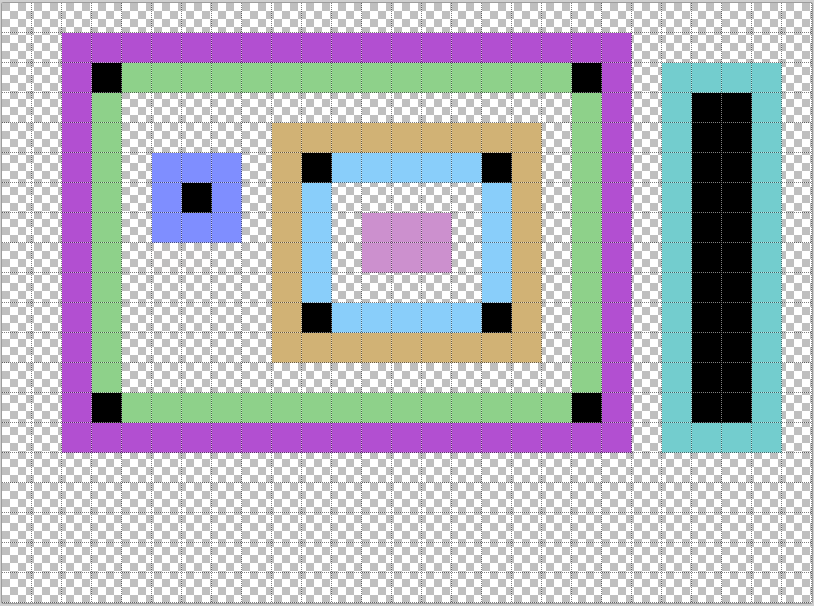
\includegraphics[scale=0.25]{SuzukiExample_contours_upscaled.png}
            \end{subfigure}
        \end{figure}
    \end{frame}
    \begin{frame}
        \frametitle{Трассировка контура. Иерархия}
        \begin{figure}[H]
            \centering
            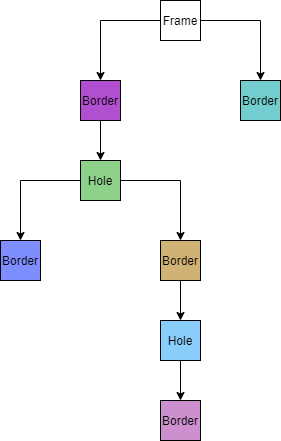
\includegraphics[scale=0.65]{SuzukiExample_hierarchy.png}
        \end{figure}
    \end{frame}
    \begin{frame}
        \frametitle{Трассировка контура. Pixels to Vertices}
        Проблемы пиксельного контура:
        \begin{itemize}
            \item Неразрешимые самопересечения
            \item Отсечение правых и нижних границ
        \end{itemize}
        \begin{figure}[H]
            \centering
            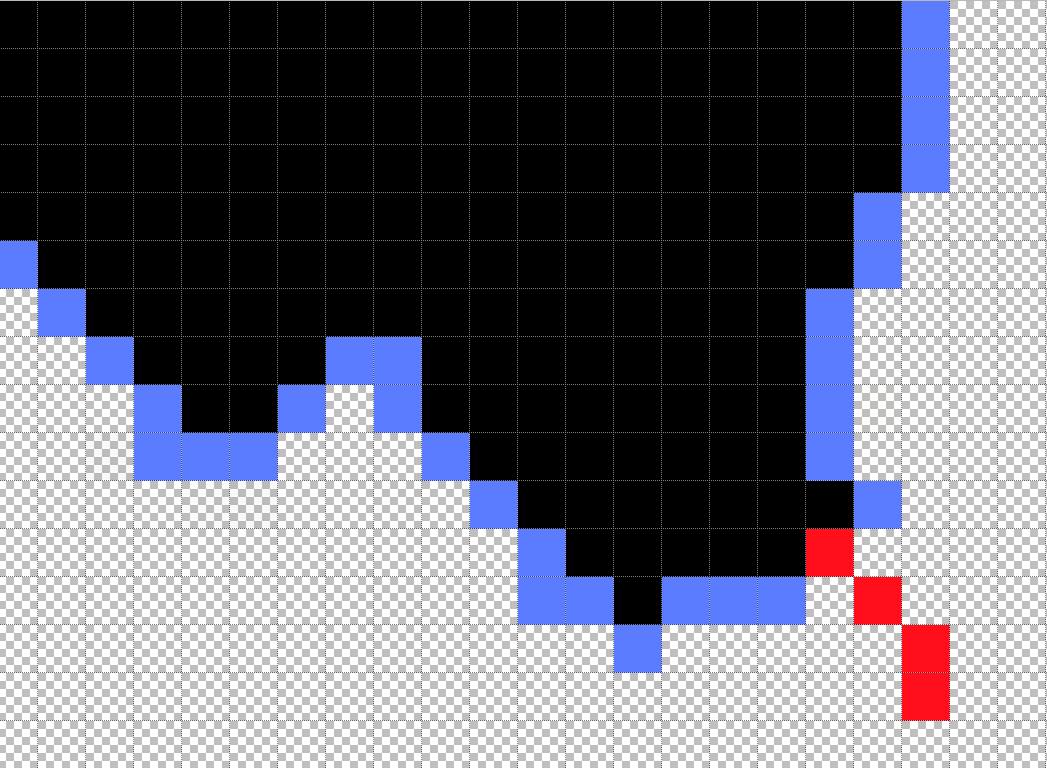
\includegraphics[scale=0.25]{SelfIntersectingContour1.png}
        \end{figure}
    \end{frame}
    \begin{frame}
        \frametitle{Трассировка контура. Pixels to Vertices}
        \begin{figure}[H]
            \centering
            \begin{subfigure}[l]{0.50\linewidth}
                \centering
                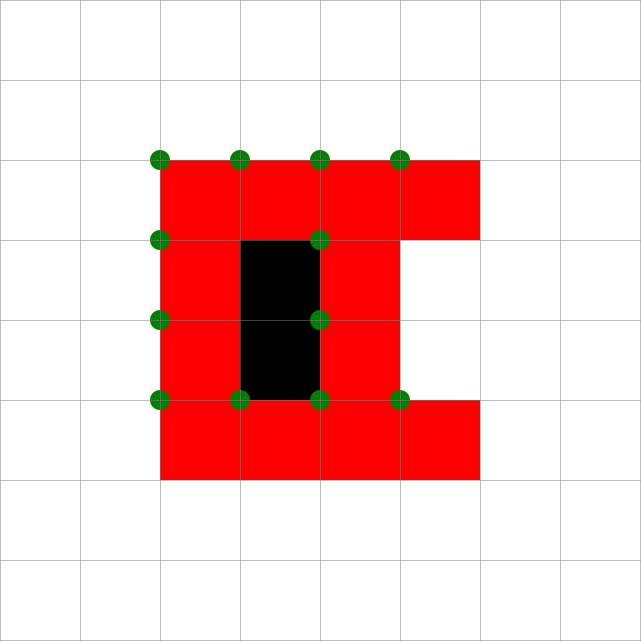
\includegraphics[scale=0.25]{SuzukiExample2_uvs.png}
            \end{subfigure}
            \begin{subfigure}{0.49\linewidth}
                \centering
                
\includegraphics[scale=0.25]{SuzukiExample2_wanted_uvs.png}
            \end{subfigure}
        \end{figure}
    \end{frame}
    \begin{frame}
        \frametitle{Трассировка контура. Первичная аппроксимация}
        \begin{figure}[H]
            \centering
            \begin{subfigure}[l]{0.50\linewidth}
                \centering
                
\includegraphics[scale=2]{donutpixel_contour_none.png}
            \end{subfigure}
            \begin{subfigure}{0.49\linewidth}
                \centering
                
\includegraphics[scale=2]{donutpixel_contour_simple.png}
            \end{subfigure}
        \end{figure}
    \end{frame}
    \begin{frame}
        \frametitle{Аппроксимация контура}
        \begin{itemize}
            \item Применение минимальных по стоимости преобразований
            \item Слияение полигонов
        \end{itemize}
        \begin{figure}[H]
            \centering
            \begin{subfigure}[l]{0.33\linewidth}
                \centering
                
\includegraphics[scale=1.5]{donutpixel_approx_start.png}
            \end{subfigure}
            \begin{subfigure}{0.33\linewidth}
                \centering
                
\includegraphics[scale=1.5]{donutpixel_approx_mid.png}
            \end{subfigure}\begin{subfigure}{0.33\linewidth}
                \centering
                
\includegraphics[scale=1.5]{donutpixel_approx_end.png}
            \end{subfigure}
        \end{figure}
    \end{frame}
    \begin{frame}
        \frametitle{Аппроксимация контура. Преобразования}
        \begin{figure}[H]
            \centering
            \begin{subfigure}[t]{\linewidth}
                \centering
                
\includegraphics[scale=0.8]{images/earcut.png}
            \end{subfigure}
            \begin{subfigure}[b]{\linewidth}
                \centering
                
\includegraphics[scale=0.8]{images/bendneighbor.png}
            \end{subfigure}
        \end{figure}
    \end{frame}
    \begin{frame}
        \frametitle{Аппроксимация контура. Преобразования}
        \begin{figure}[H]
            \centering
            
\includegraphics[scale=0.8]{images/remove_triangular_hole.png}
        \end{figure}
    \end{frame}
    \begin{frame}
        \frametitle{Аппроксимация контура. Преобразования}
        \begin{figure}[H]
            \begin{subfigure}[t]{\linewidth}
                \centering
                
\includegraphics[scale=0.8]{images/bendneighbor2.png}
            \end{subfigure}
            \begin{subfigure}[t]{\linewidth}
                \centering
                
\includegraphics[scale=0.8]{images/bendoutboth.png}
            \end{subfigure}
        \end{figure}
    \end{frame}
    \begin{frame}
        \frametitle{Аппроксимация контура. Слияние}
        \begin{figure}[H]
            \centering
            \begin{subfigure}[t]{\linewidth}
                \centering
                
\includegraphics[scale=0.8]{images/polygonmerge.png}
            \end{subfigure}
            \begin{subfigure}[t]{\linewidth}
                \centering
                
\includegraphics[scale=0.8]{images/polygonmerge2.png}
            \end{subfigure}
        \end{figure}
    \end{frame}
    \begin{frame}
        \frametitle{Аппроксимация контура}
        Стоимость преобразования -- добавочная площадь
        \begin{itemize}
            \item Дерево полигонов с корнем в рамке изображения
            \item Триангуляция Делоне с ограничениями для проверки преобразований
            \item BST для поиска вершины с минимальной стоимостью преобразования
        \end{itemize}
    \end{frame}
    \begin{frame}
        \frametitle{Аппроксимация контура. Алгоритм слияния}
        \begin{figure}[H]
            \centering
            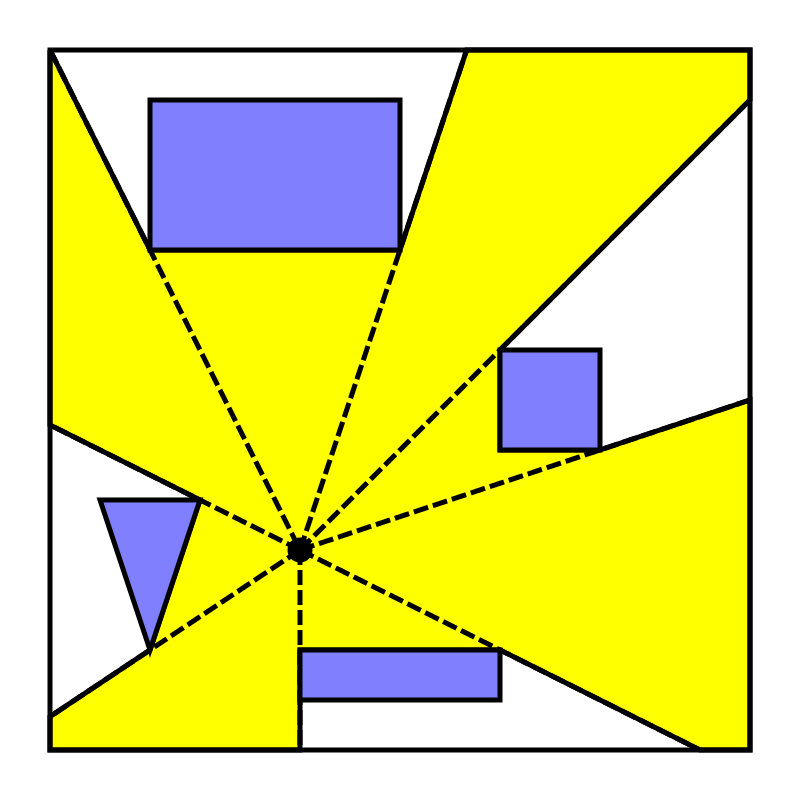
\includegraphics[scale=0.3]{visibility_polygon.png}
        \end{figure}
    \end{frame}
    \begin{frame}
        \frametitle{Аппроксимация контура. Алгоритм слияния}
        Triangular Expansion $O\left(nh\right)$ нахождение полигона видимости
        $O\left(\log_2\left|V\right|\right)$ на запрос нахождения точки в полигоне видимости
        \begin{figure}[H]
            \centering
            \begin{subfigure}[t]{0.49\linewidth}
                \centering
                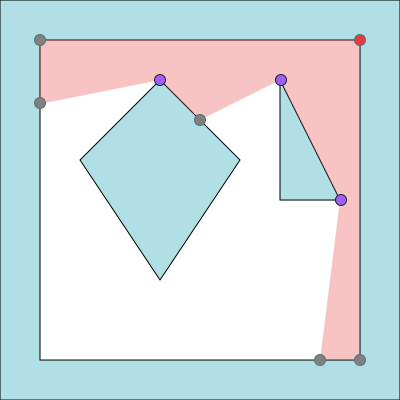
\includegraphics[scale=0.4]{visibility_polygon_prev_vertex.png}
            \end{subfigure}
            \begin{subfigure}[t]{0.49\linewidth}
                \centering
                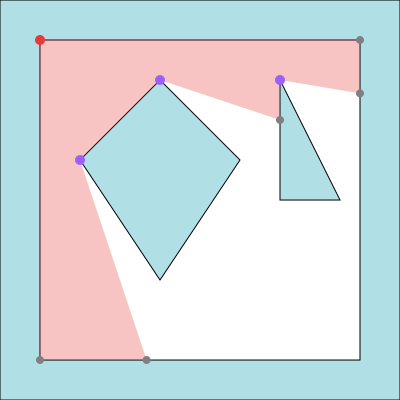
\includegraphics[scale=0.4]{visibility_polygon_current_vertex.png}
            \end{subfigure}
        \end{figure}
    \end{frame}
    \begin{frame}
        \frametitle{Генерация меша}
        DFS. Структурные ребра это вход в полигон или выход из него
        \begin{figure}[H]
            \centering
            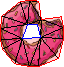
\includegraphics[scale=1.5]{donutpixel_mesh.png}
        \end{figure}
    \end{frame}
    \begin{frame}
        \frametitle{Упаковка в атлас. Генетический алгоритм}
        \begin{center}
            \begin{algorithmic}[1]
                \State $INITIALIZE$ population with random candidate solution
                \State $EVALUATE$ each candidate
                \While{$TERMINATION\; CONDITION$ \textbf{is not} satisfied}
                    \State $SELECT$ parents
                    \State $RECOMBINE$ pairs of parents
                    \State $MUTATE$ offspring
                    \State $EVALUATE$ new candidates
                    \State $SELECT$ individuals for the next generation
                \EndWhile
            \end{algorithmic}
        \end{center}
    \end{frame}
    \begin{frame}
        \frametitle{Генетический алгоритм. Репрезентация особей}
        \begin{figure}[H]
            \centering
            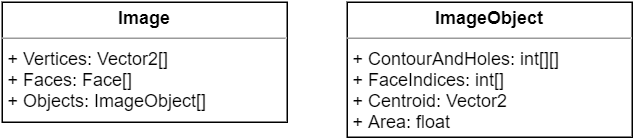
\includegraphics[scale=0.8]{Image.png}
        \end{figure}
    \end{frame}
    \begin{frame}
        \frametitle{Генетический алгоритм. Репрезентация особей}
        \begin{itemize}
            \item Массив троек (X, Y, Angle) для каждого ImageObject
            \item Массив булевых флагов присутствия в атласе для каждого Image
        \end{itemize}
    \end{frame}
    \begin{frame}
        \frametitle{Генетический алгоритм. Операторы рекомбинации}
        Мутации:
        \begin{itemize}
            \item Creep
            \item Reset
        \end{itemize}
        One Point Crossover
        \begin{figure}[H]
            \centering
            
\includegraphics[scale=1]{OnePointCrossover.png}
        \end{figure}
    \end{frame}
    \begin{frame}
        \frametitle{Генетический алгоритм. Выбор родителей}
        Stochastic Universal Sampling:
        \begin{center}
            \scalebox{0.80}{
                \begin{minipage}{\linewidth}
                    \begin{algorithmic}[1]
                        \State $a$ is cumulative probability distribution
                        \State $m$ is number of parents we want to selects
                        \State $current \gets 1$
                        \State $i \gets 1$
                        \State $r \gets$ uniformly random from $\left[0, 1 / m\right]$
                        \While{$current \leq m$}
                            \While{$r \leq a_i$}
                                \State $parents_i \gets popoluation_i$
                                \State $r \gets r + 1 / m$
                                \State $current \gets current + 1$
                            \EndWhile
                            \State $i \gets i + 1$
                        \EndWhile
                    \end{algorithmic}
                \end{minipage}
            }
        \end{center}
        Экспоненциальный ранг:
        \[P_{exp}\left(i\right) = \frac{1 - e^{-i}}{c}\]
    \end{frame}
    \begin{frame}
        \frametitle{Генетический алгоритм. Отбор выживших}
        \begin{itemize}
            \item Elitism
            \item Age based
            \item GENITOR -- замещение худших
        \end{itemize}
    \end{frame}
    \begin{frame}
        \frametitle{Генетический алгоритм. Функция оценки}
        \[
            F\left(individual\right) = a \cdot S_{intersection} + b \cdot S_{outside\;ledges} + c \cdot missing \cdot S_{avg}
        \]
        \begin{figure}[H]
            \centering
            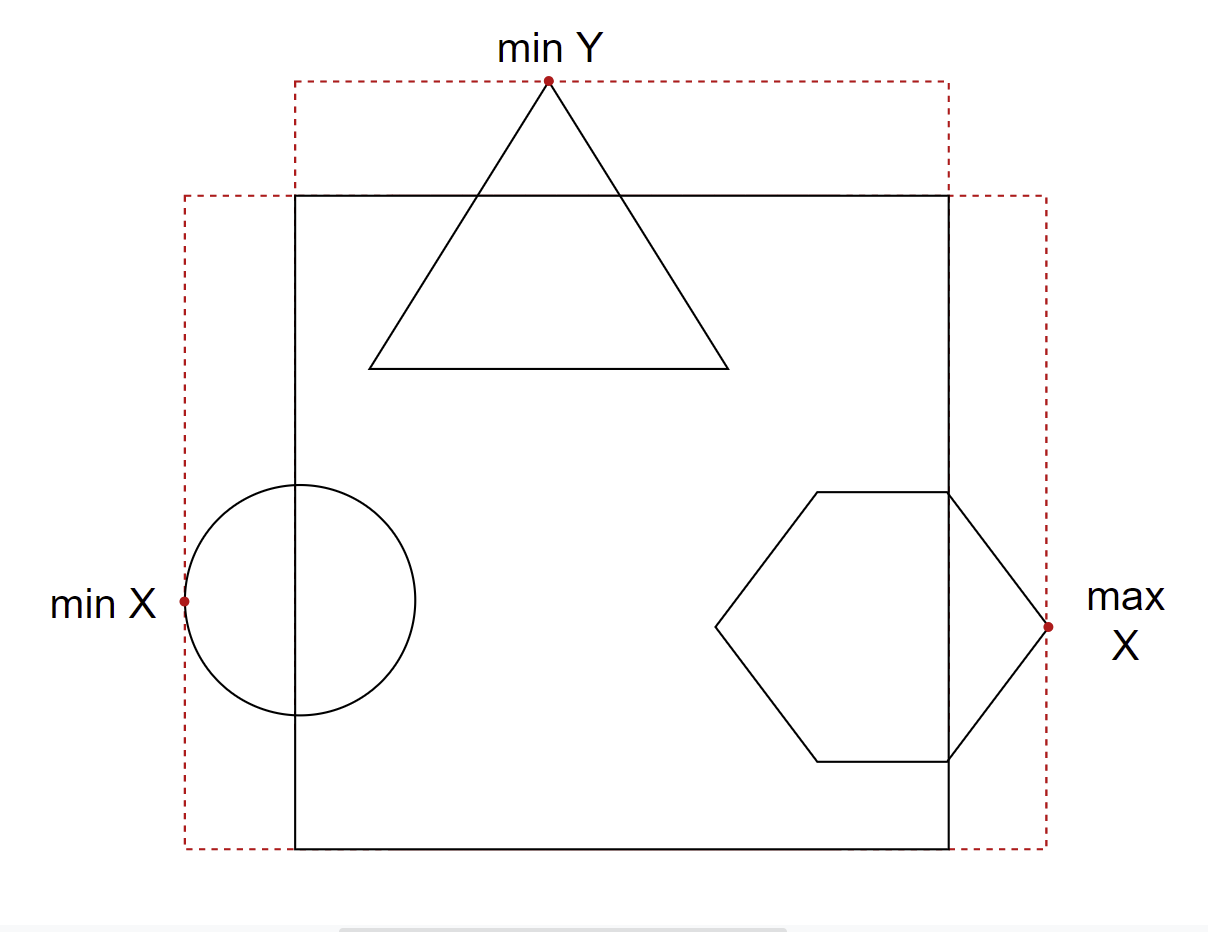
\includegraphics[scale=0.25]{ledges.png}
        \end{figure}
    \end{frame}
    \begin{frame}
        \frametitle{Генетический алгоритм. Функция оценки}
        \[
            S_{intersection} = \sum\limits_{0}^{n - 1}S\left(P_i\right) - S\left(\bigcup\limits_{0}^{n - 1}P_i\right)
        \]
        Clipper library by Angus Johnson (extended Vatti)
    \end{frame}
    \begin{frame}
        \frametitle{Memetic algorithm}
        \begin{itemize}
            \item Hole filler
            \item Physics (Box2D)
        \end{itemize}
    \end{frame}
    \begin{frame}
        \frametitle{Генетический алгоритм. Пример работы}
        \begin{table}[ht]
            \begin{center}
            \begin{tabular}{cc}
                \multirow{2}{*}[2cm]{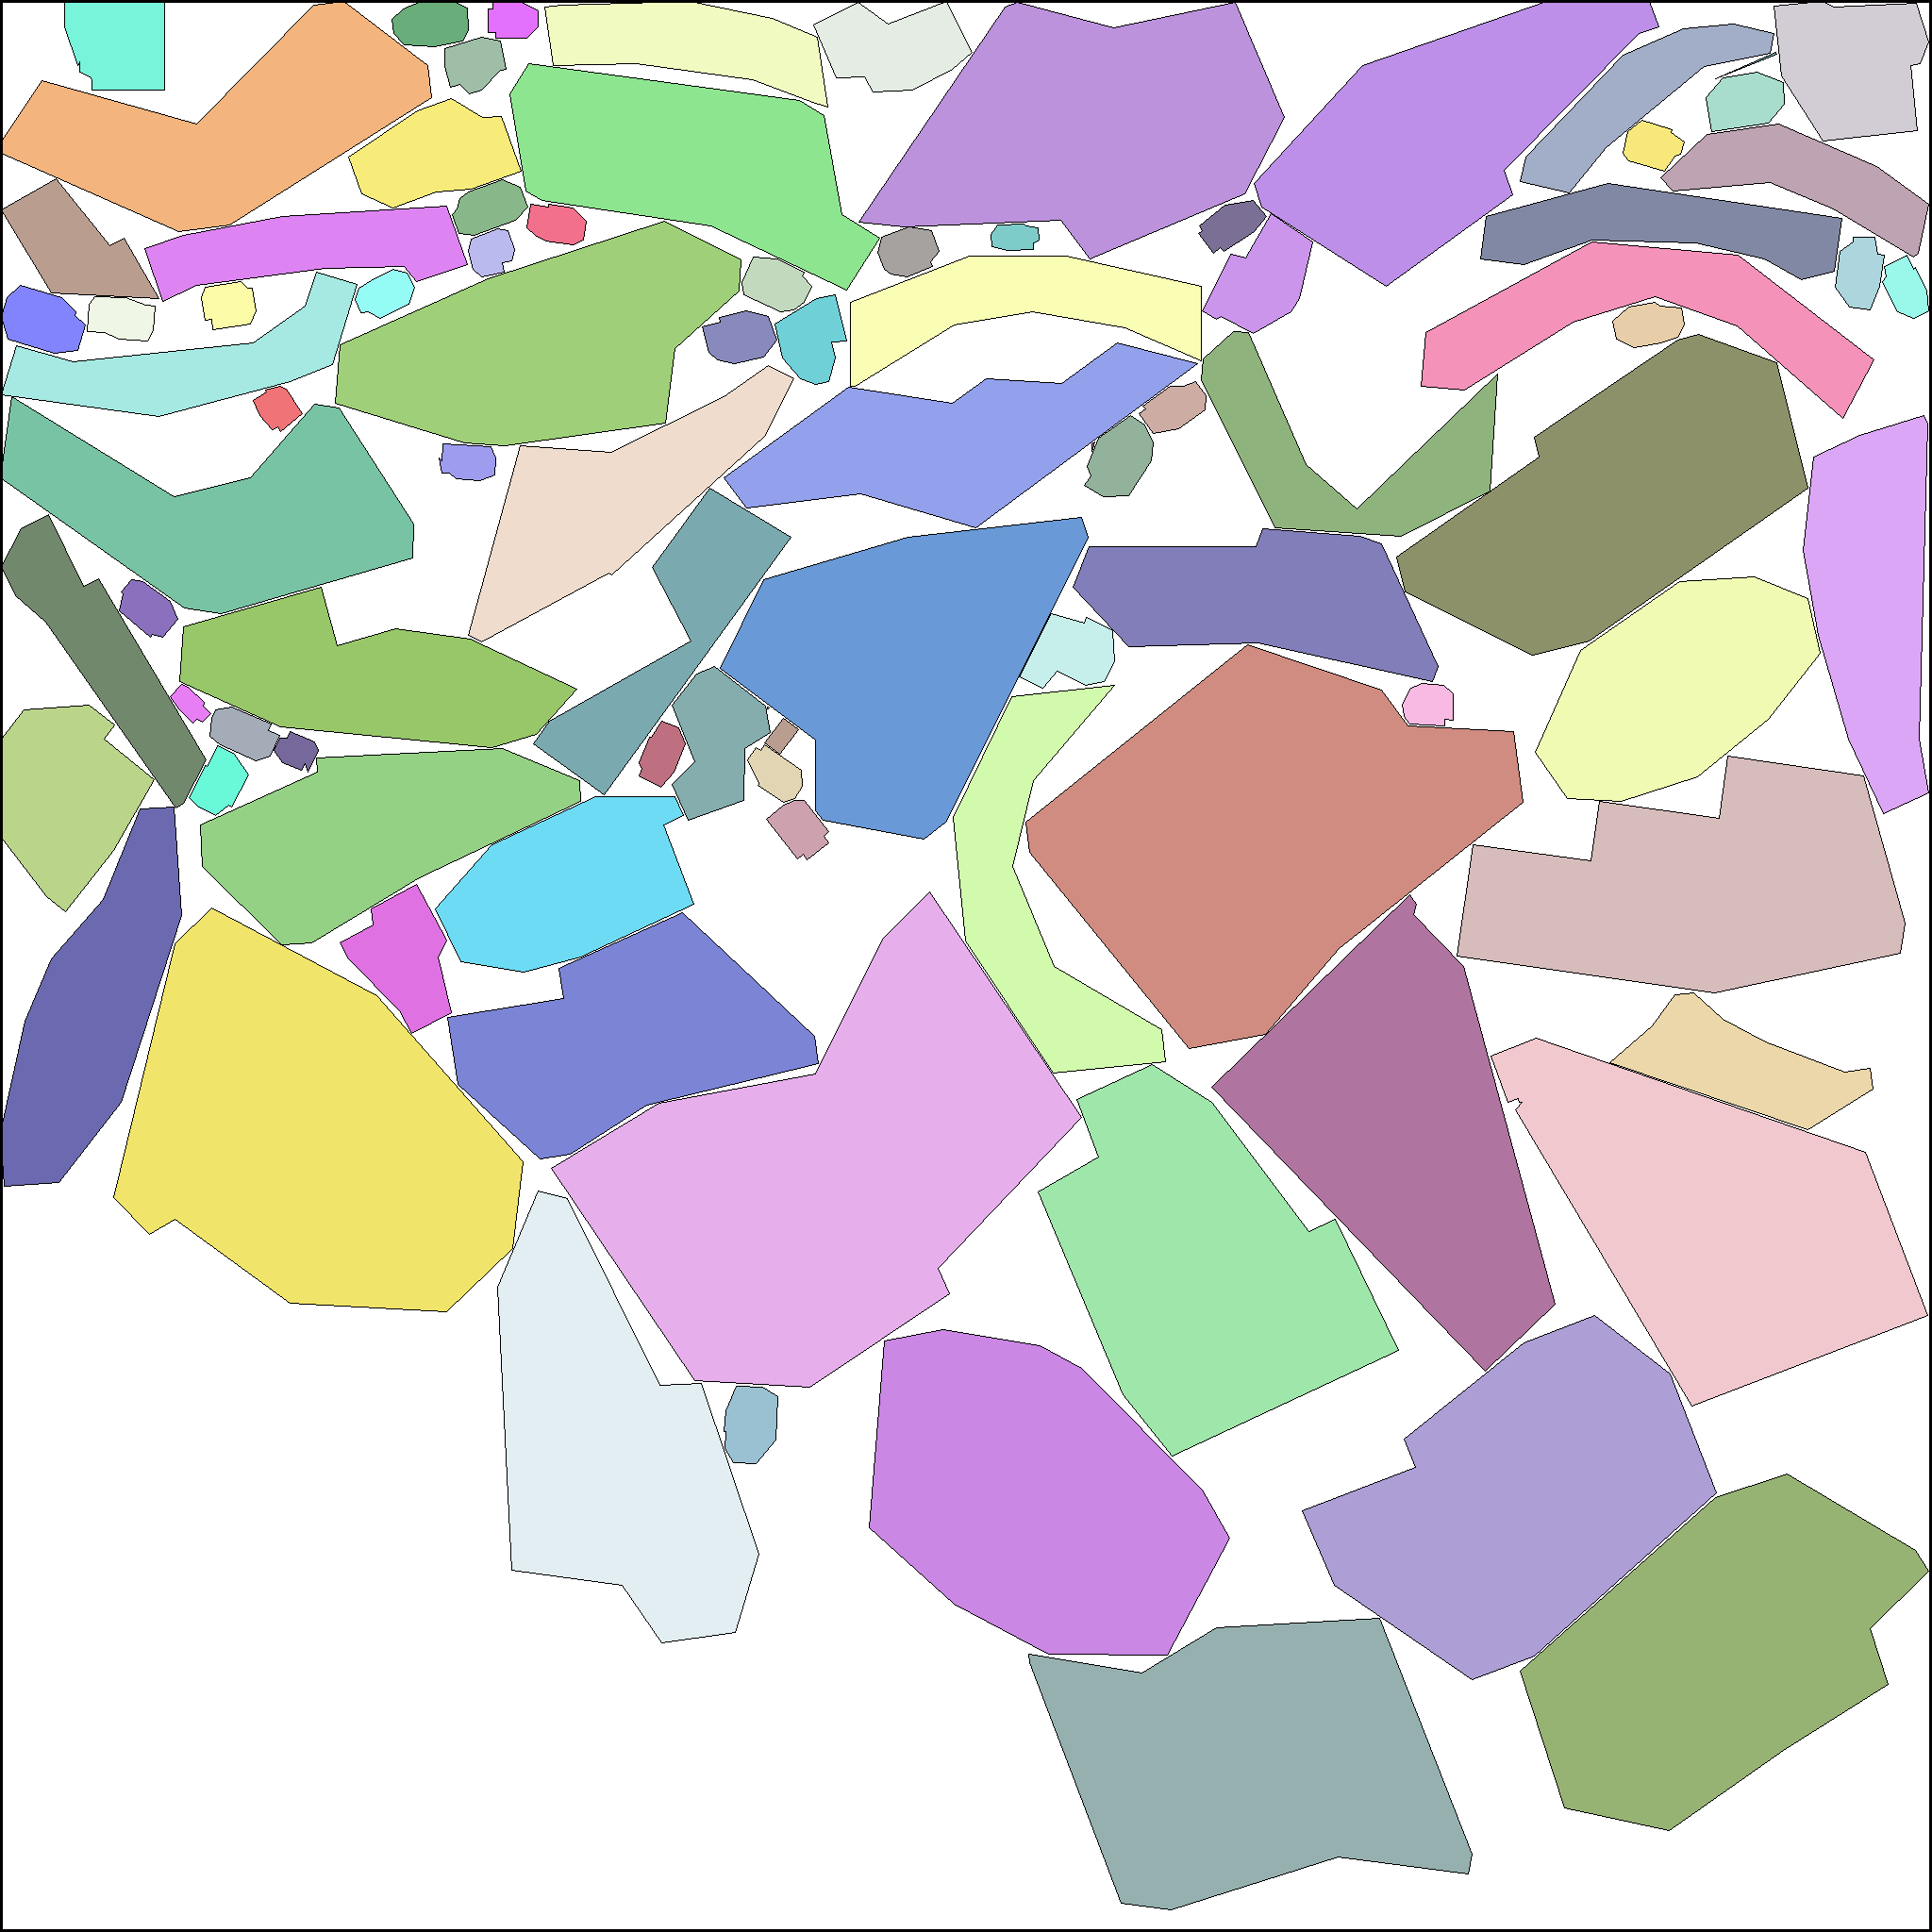
\includegraphics[scale=0.08]{polygonal.png}}&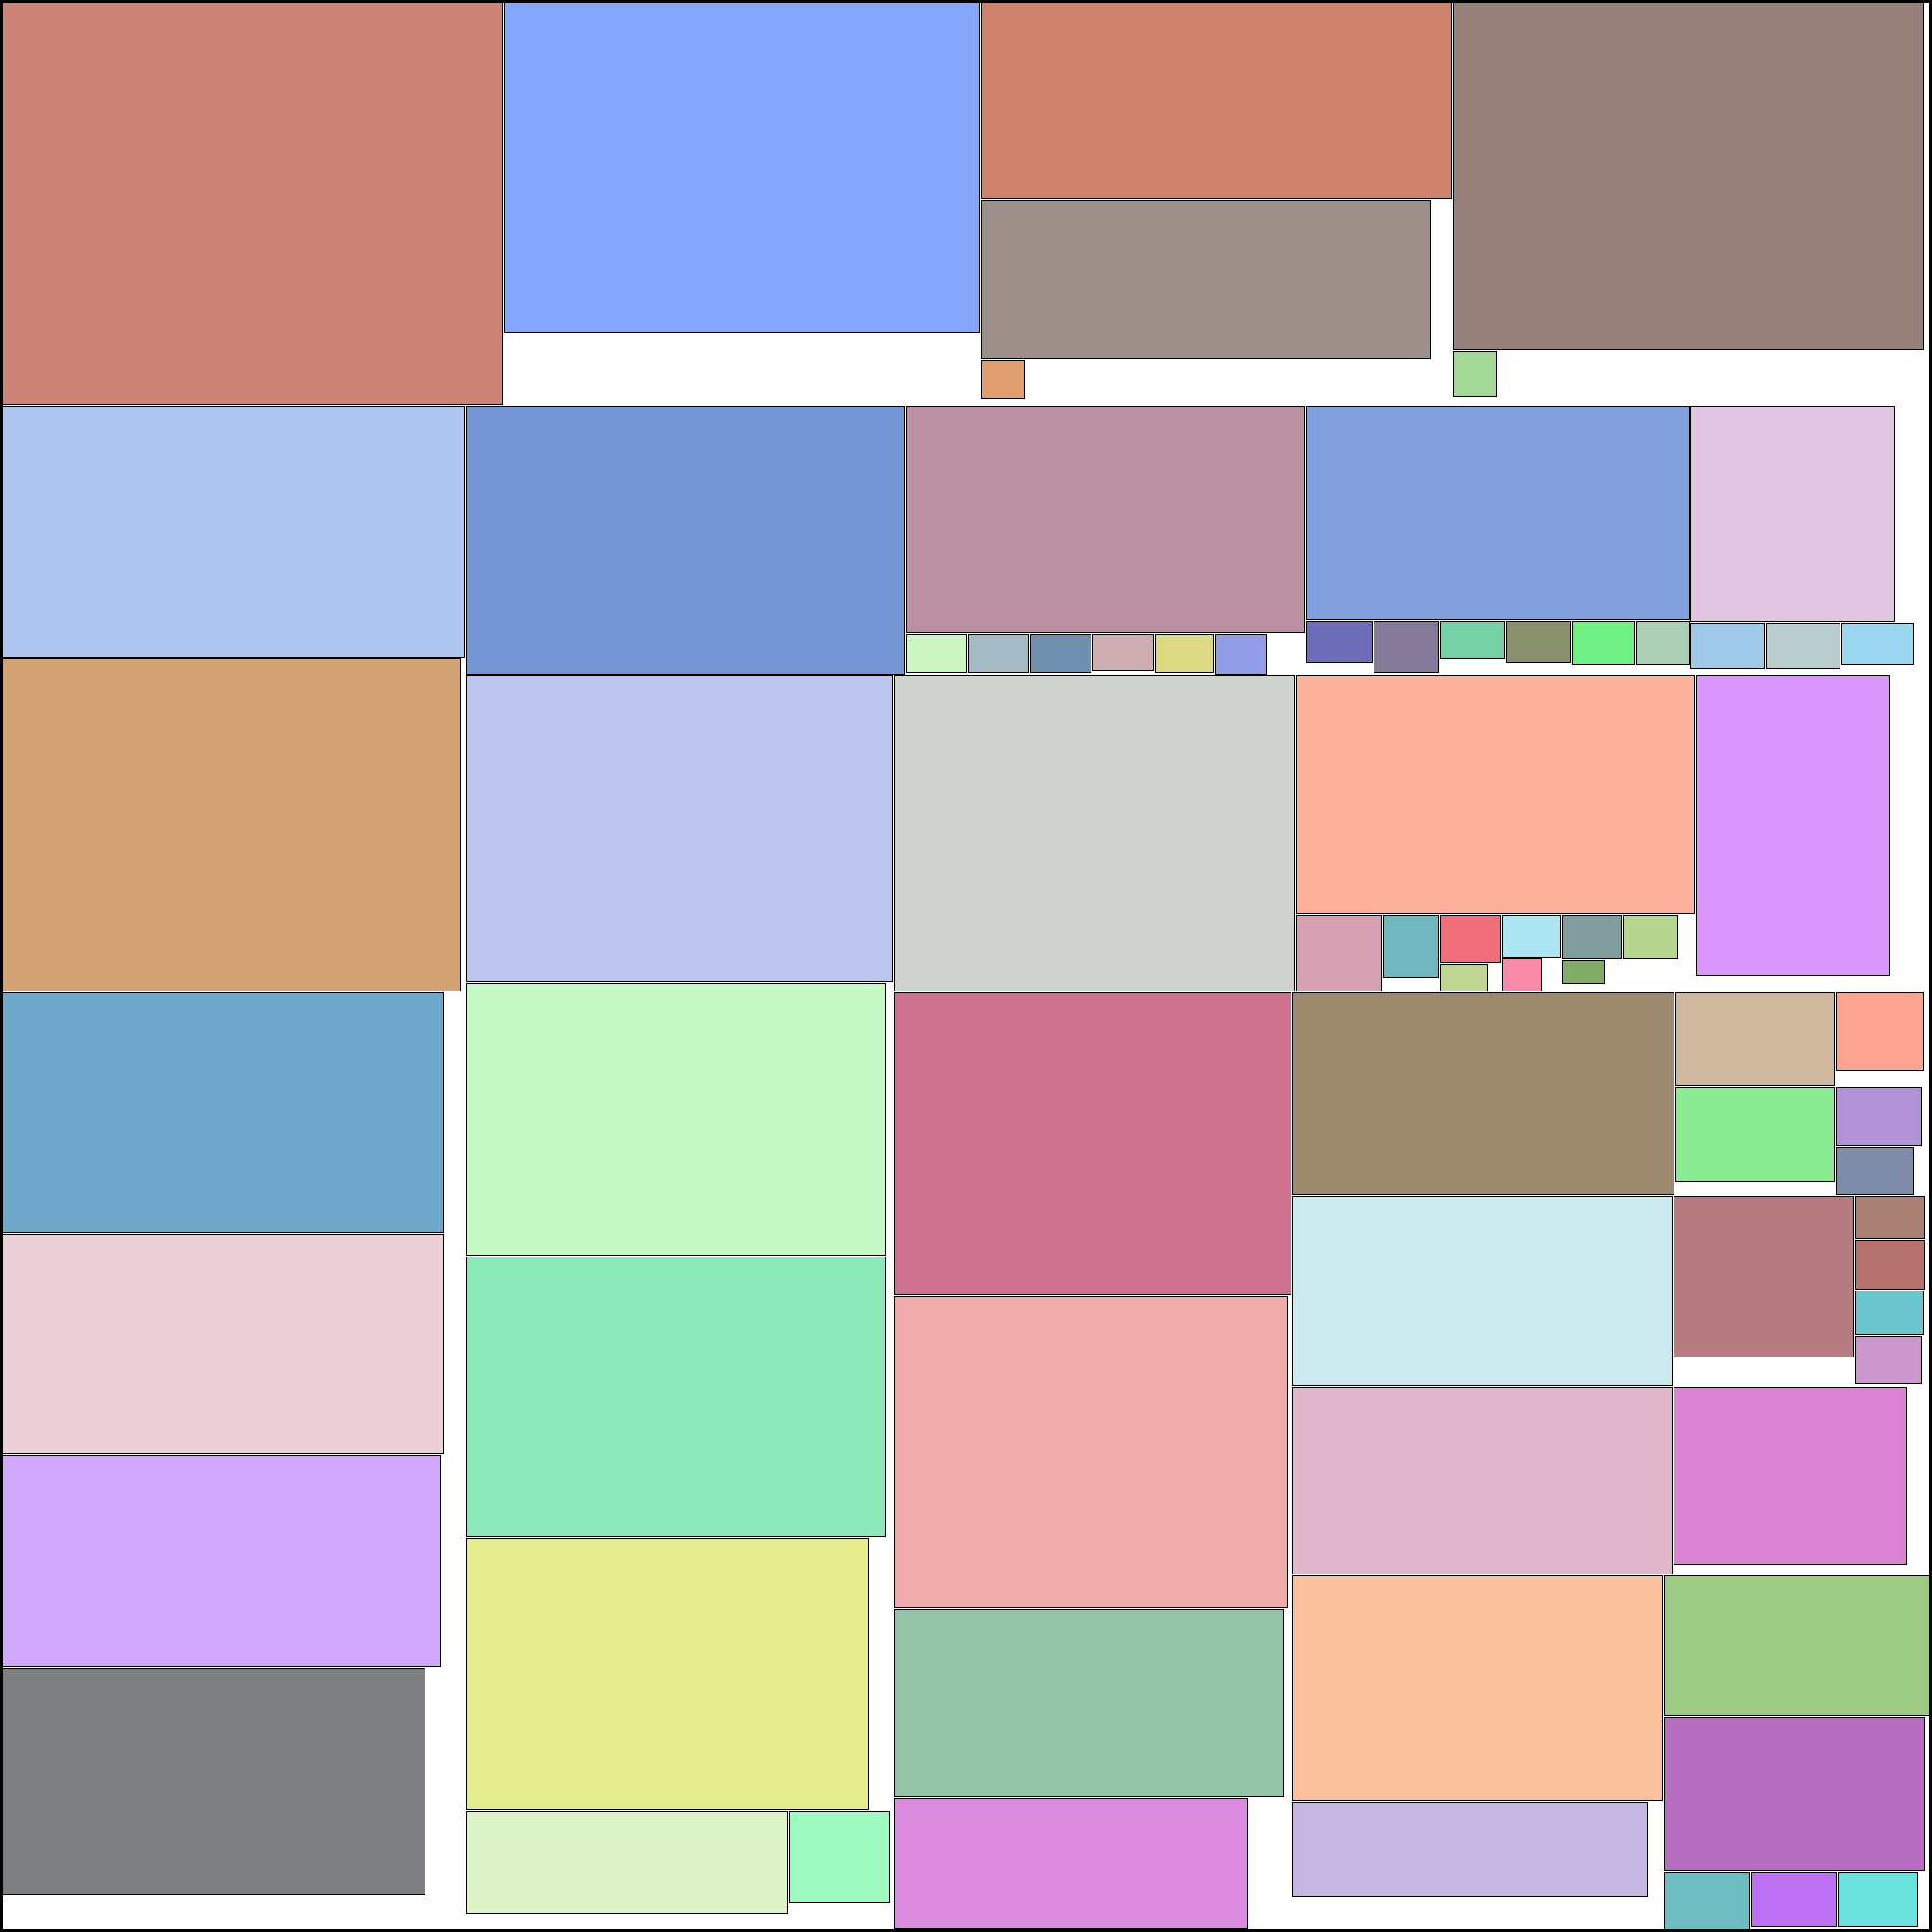
\includegraphics[scale=0.08]{rect_0.png}\\
                &
\includegraphics[scale=0.08]{rect_1.png}
            \end{tabular}
            \end{center}
        \end{table}
    \end{frame}
\end{document}
